\section{Results and Discussion}

\subsection{RHESSI Hard X-rays}\label{rhessiresults}
%RHESSI
\begin{figure}[H]
  \begin{center}
  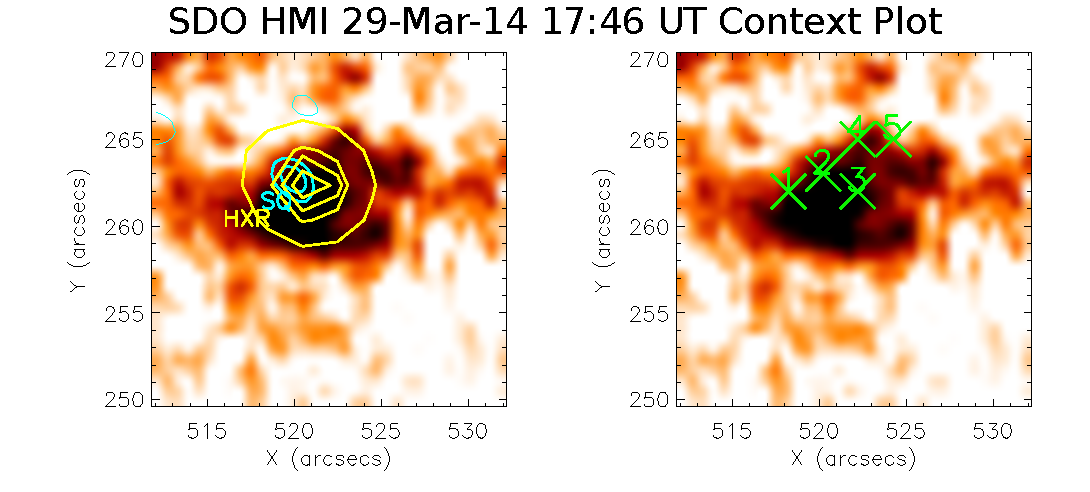
\includegraphics[width=0.9\textwidth]{29-Mar-14-HMI-Sunquake-Context-Plot}
  \end{center}
  \caption{The images show SDO HMI continuum data in reverse colour scheme; with the left image displaying yellow contours representing 50 to 100 keV HXR emission at 80, 90, 92, 94, 96 and 98$\%$ of maximum and 6mHz sunquake power in cyan; the right image shows sample coordinates as green crosses with their associated number relating to Table \ref{coordtab}. Each of the IRIS SJ, IRIS SG and SDO HMI data sets are sampled at the exact same coordinates in heliocentric units.}\label{hmicontext}
\end{figure}


For a sunquake to be generated by accelerated particle collision then the incident beam must be aligned over the acoustic impact location \citep{1998IAUS..185..191K}. To investigate this spatial alignment, RHESSI 50 to 100 keV HXR and sunquake egression power contours are plotted on a reverse colour, filtered HMI continuum image shown in Figure \ref{hmicontext}. The contours show a reasonable alignment but a more rigorous way to test the spatial and temporal relationship between nonthermal electrons, sunquake and other emission is to analyse lightcurves from the region of interest.   %explain alignment of different faetures and the significance      
%need to run hmi_context_plot.pro

RHESSI HXR data are taken from central coordinates 518" by 262", sampling the sunquake epicentre. When the data are fit to a nonthermal electron model, a spectrum is produced which can be used to plot the energy curve shown in Figure \ref{erhessi}. The chi-squared, $\chi^{2}$, of the fit can be seen in Figure \ref{chi}. $\chi^{2} = 0$ means an exact match to the model, whereas $\chi^{2} > 0$ means the fit deviates. However, in general, a $\chi^{2} < 5$ means the data fits well to the theoretical model. The plot in Figure \ref{erhessi} shows 10 - 100 keV nonthermal power over time. The impulsive phase of the flare is visible from 17:46, peaking at 17:47, with the plot showing a double peak profile which climbs from $1.0{\times}10^{28}$ to $2.5{\times}10^{29}$ erg. 



\begin{figure}[H]
  \begin{center}
  \textbf{RHESSI 10 - 100 keV Hard Xray Energy Over Time}\par\medskip
  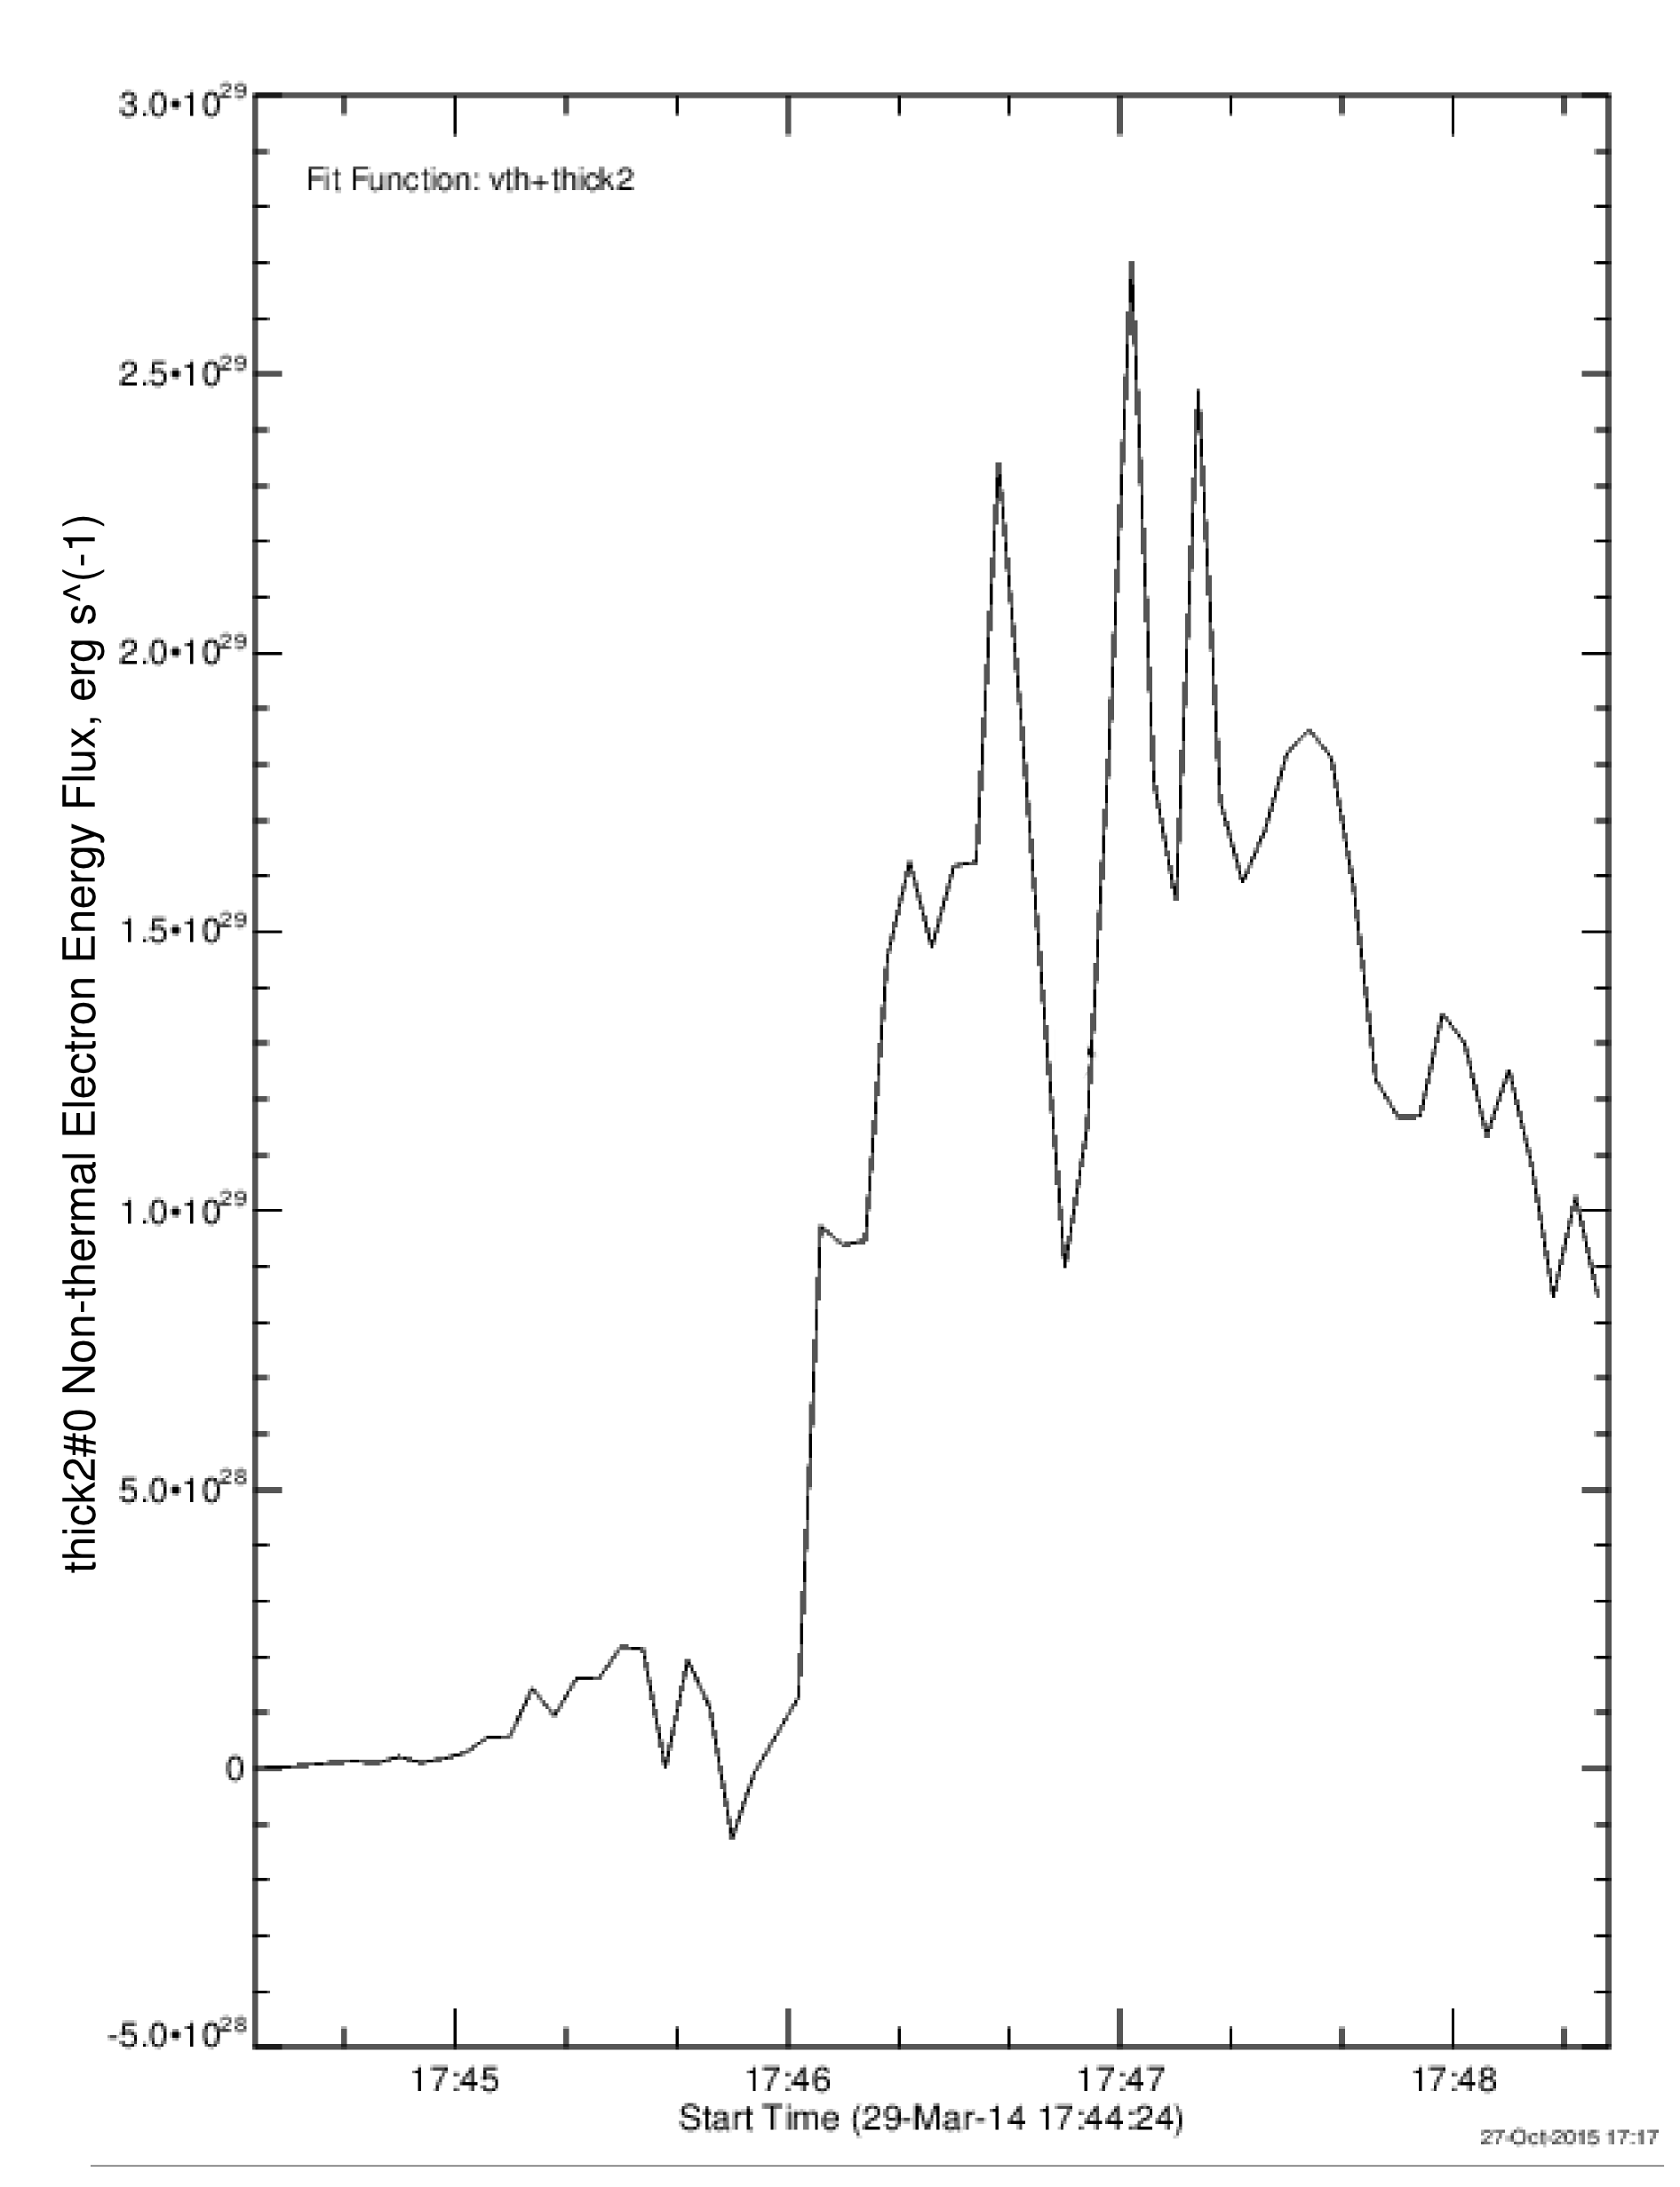
\includegraphics[width=0.9\textwidth]{rhessi-energy-curve}
  \end{center}
  \caption{Shows the energy evolution of hard x-ray emission collected by RHESSI 10 to 100 keV bins over the sunquake region (518", 262"). HXR emission is due to non-thermal electrons, thus energy is calculated by fitting data to the collisional thick target model. The HXRs impulsive phase begins at around 17:46 and peaks at 17:47, showing temporal alignment with IRIS and HMI datasets shown in Figure \ref{fluxladder}.}
\end{figure}\label{erhessi}



\begin{figure}[H]
  \begin{center}
  \textbf{Chi Squared for RHESSI 10 - 100 keV Hard Xray Fit}\par\medskip
  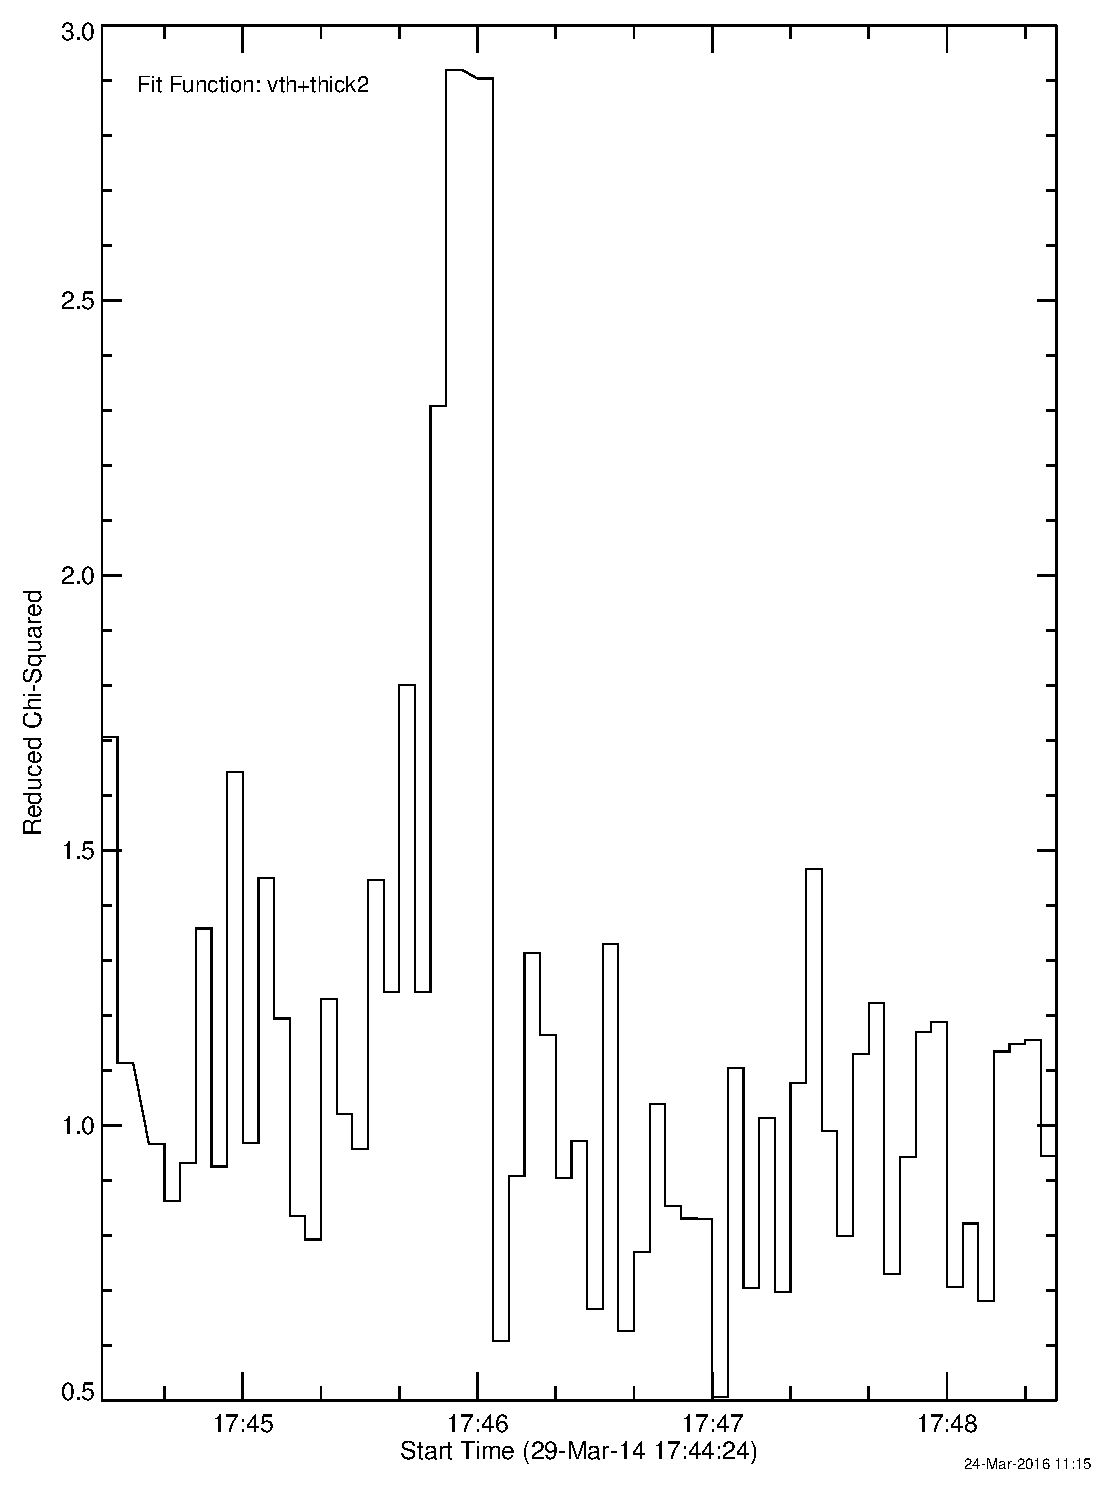
\includegraphics[width=0.9\textwidth]{rhessi-10-100-kev-fit-chi-squared}
  \end{center}
  \caption{Shows the Chi squared for the nonthermal fit performed on RHESSI 10 - 100 keV HXR data.}
\end{figure}\label{chi}


\subsection{Emission Captured By IRIS and HMI}
%LADDER PLOTS
\begin{figure}[H]
  \begin{center}
  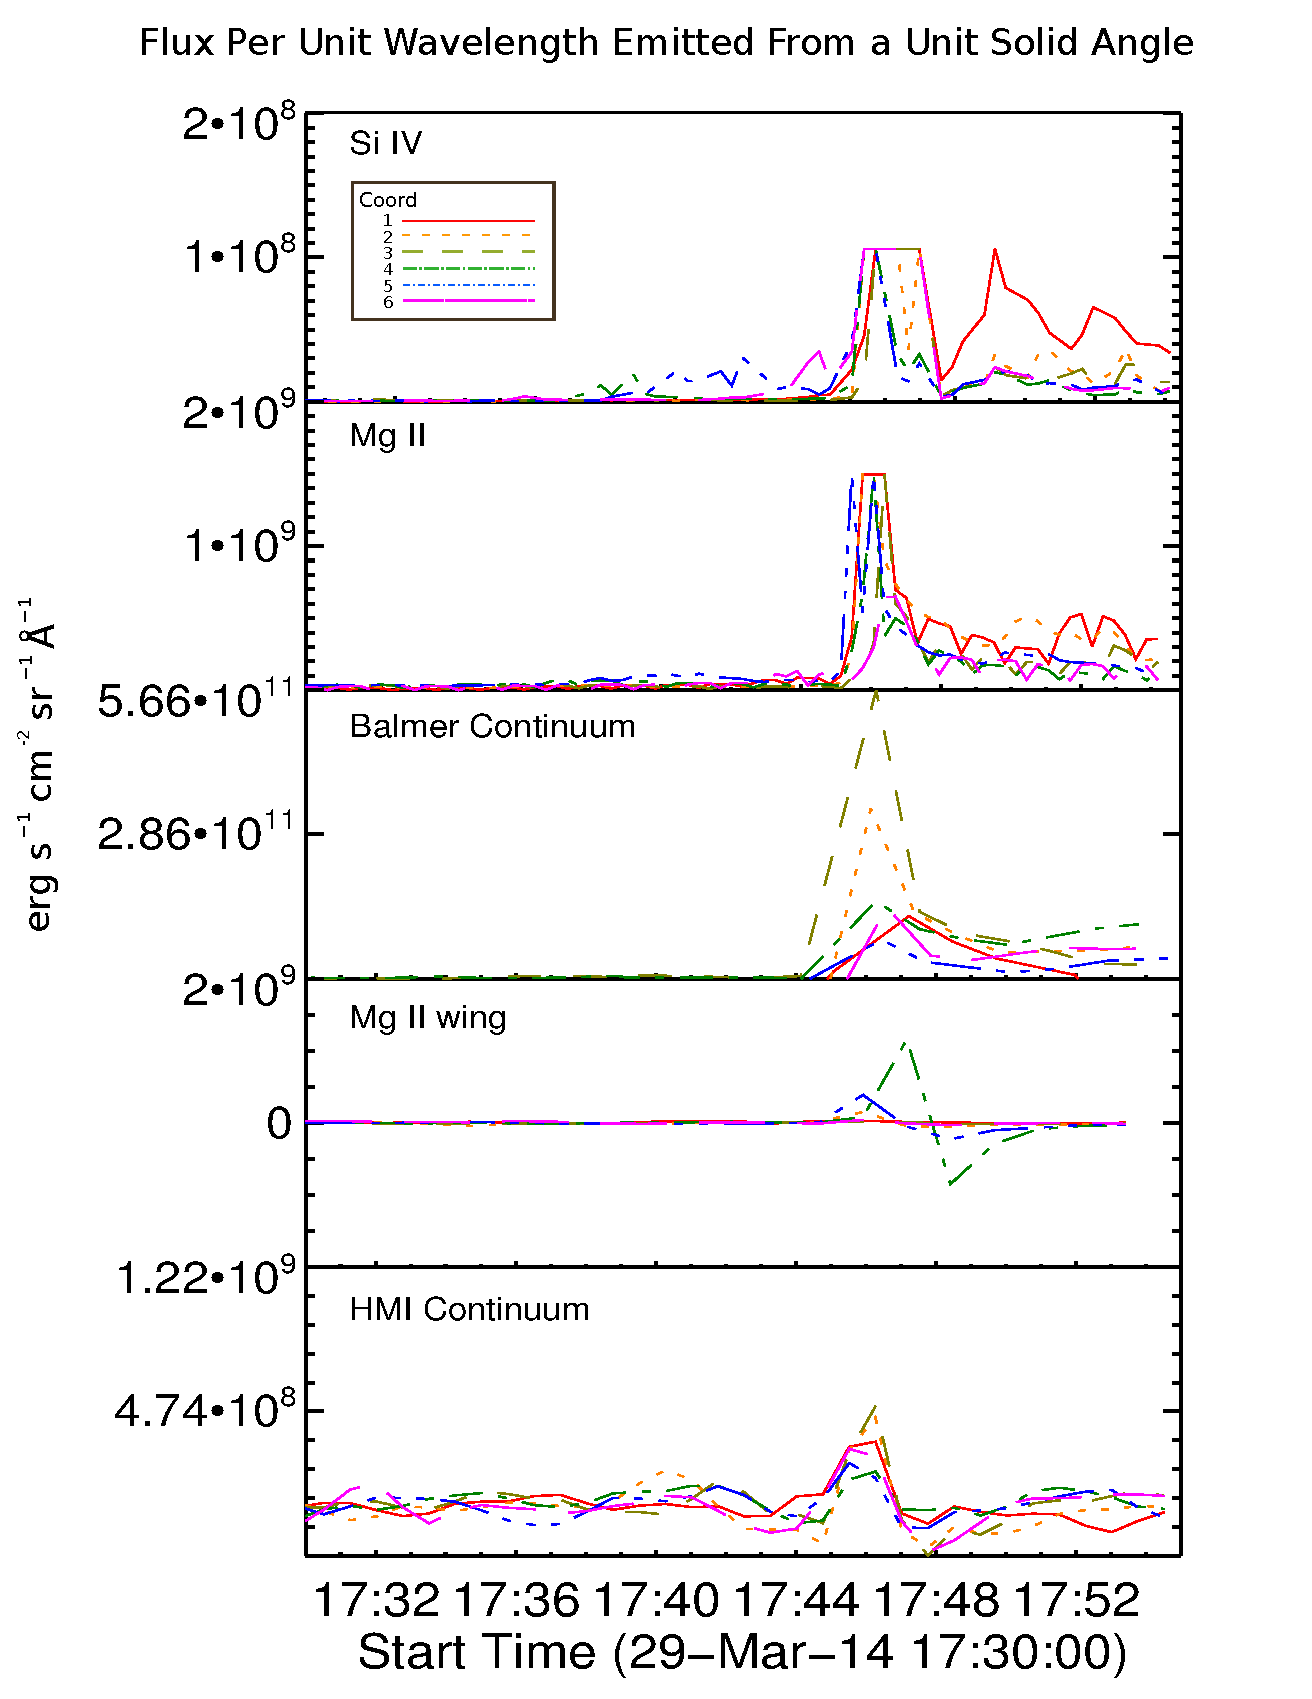
\includegraphics[width=0.85\textwidth]{29-Mar-14-Flux-Ladder}
  \end{center}
  \caption{Shows flux per wavelength from a unit solid angle or intensity. The six lines (see legend) represent areas centred on regions 1 to 6, relating to heliocentric coordinates shown in Table \ref{coordtab}. The solid red line is directly over the sunquake location. Each plot represents an independent data set, in order from top to bottom the sets are; IRIS SJ 1400 \AA\ (Si IV); IRIS SJ 2796 \AA\ (Mg II); IRIS SG  2825.7 to 2825.8 \AA\ (Balmer Continuum); IRIS SJ 2832 \AA\ (Mg II wing); SDO HMI continuum.}\label{fluxladder}
\end{figure}




\begin{figure}[H]
  \begin{center}
  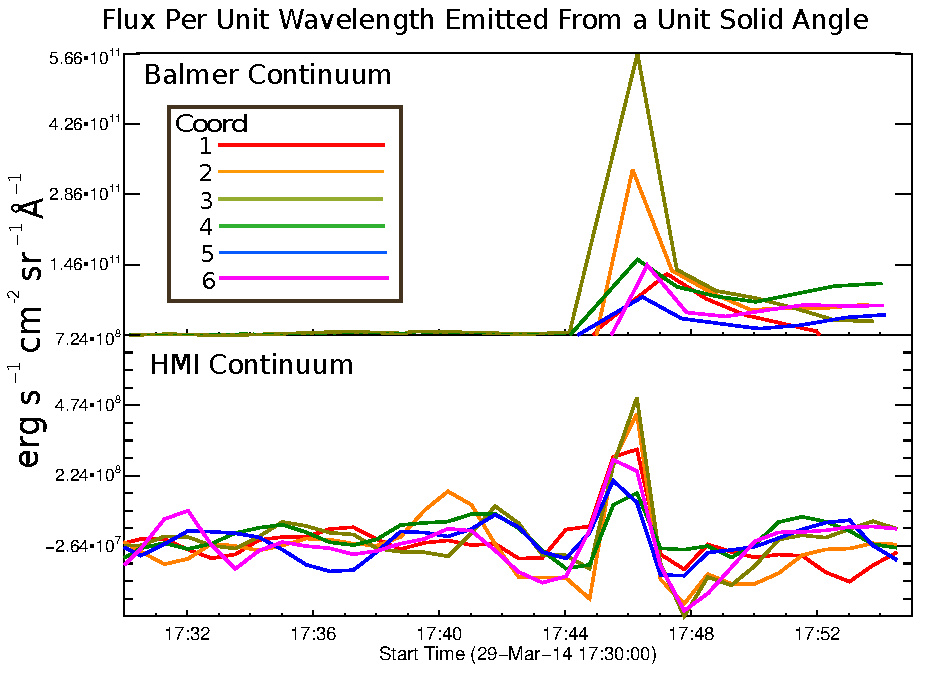
\includegraphics[width=0.9\textwidth]{29-Mar-14-Flux-Ladder-Balm-HMI-Only}
  \end{center}
  \caption{Shows flux per wavelength from a unit solid angle. The six lines (see legend) represent areas centred on regions 1 to 6, relating to heliocentric coordinates shown in Table \ref{coordtab}. The solid red line is directly over the sunquake location. Each plot represents an independent data set, in order from top to bottom the sets are; IRIS SJ 1400 \AA\ (Si IV); IRIS SJ 2796 \AA\ (Mg II); IRIS SG  2825.7 to 2825.8 \AA\ (Balmer Continuum); IRIS SJ 2832 \AA\ (Mg II wing); SDO HMI continuum.}\label{fluxladder-balm-hmi-only}
\end{figure}

%Si IV, Mg II, Balmer, MG II w, HMI
Shown in Figure \ref{fluxladder} are lightcurves of emission from the lower solar atmosphere, captured by IRIS and SDO HMI. From top to bottom the plot shows data from IRIS SJ Si IV, IRIS SJ Mg II, IRIS SG Balmer Continuum, IRIS SJ Mg II wing and SDO HMI visible continuum sampled from six coordinates in the flare ribbon. Si IV and Mg II IRIS SJ data, show a distinct cutoff which is caused by over saturation of the instrument CCD, meaning flux measurements during the impulsive phase are a lower estimate. Si IV and Mg II lightcurves are unreliable in the lack of data over the impulsive phase, however, all other datasets show a synchronised impulsive peak, with the exception of MG II wing where only coordinates four and five exhibit a significant enhancement. The red solid line in each data set is sampled from the sunquake location. At first glance the sunquake location in the plots does not seem to have any obvious differences other than a slight time delay in peak Balmer continuum emission. The delay appears to be around 45 seconds after the impulsive phase peak at approximately 17:48 which coincides with the sunquake onset time in certain frequencies \citep{2015ApJ...812...35M}. However, because of the way sunquake onset time is calculated there could be up to a five minute uncertainty. Mg II wing data shows no enhancement over the sunquake location. HMI continuum shows significant enhancement over the sunquake, which is aligned in time with the impulsive phase. 



%\begin{figure}[H]
%  \begin{center}
%  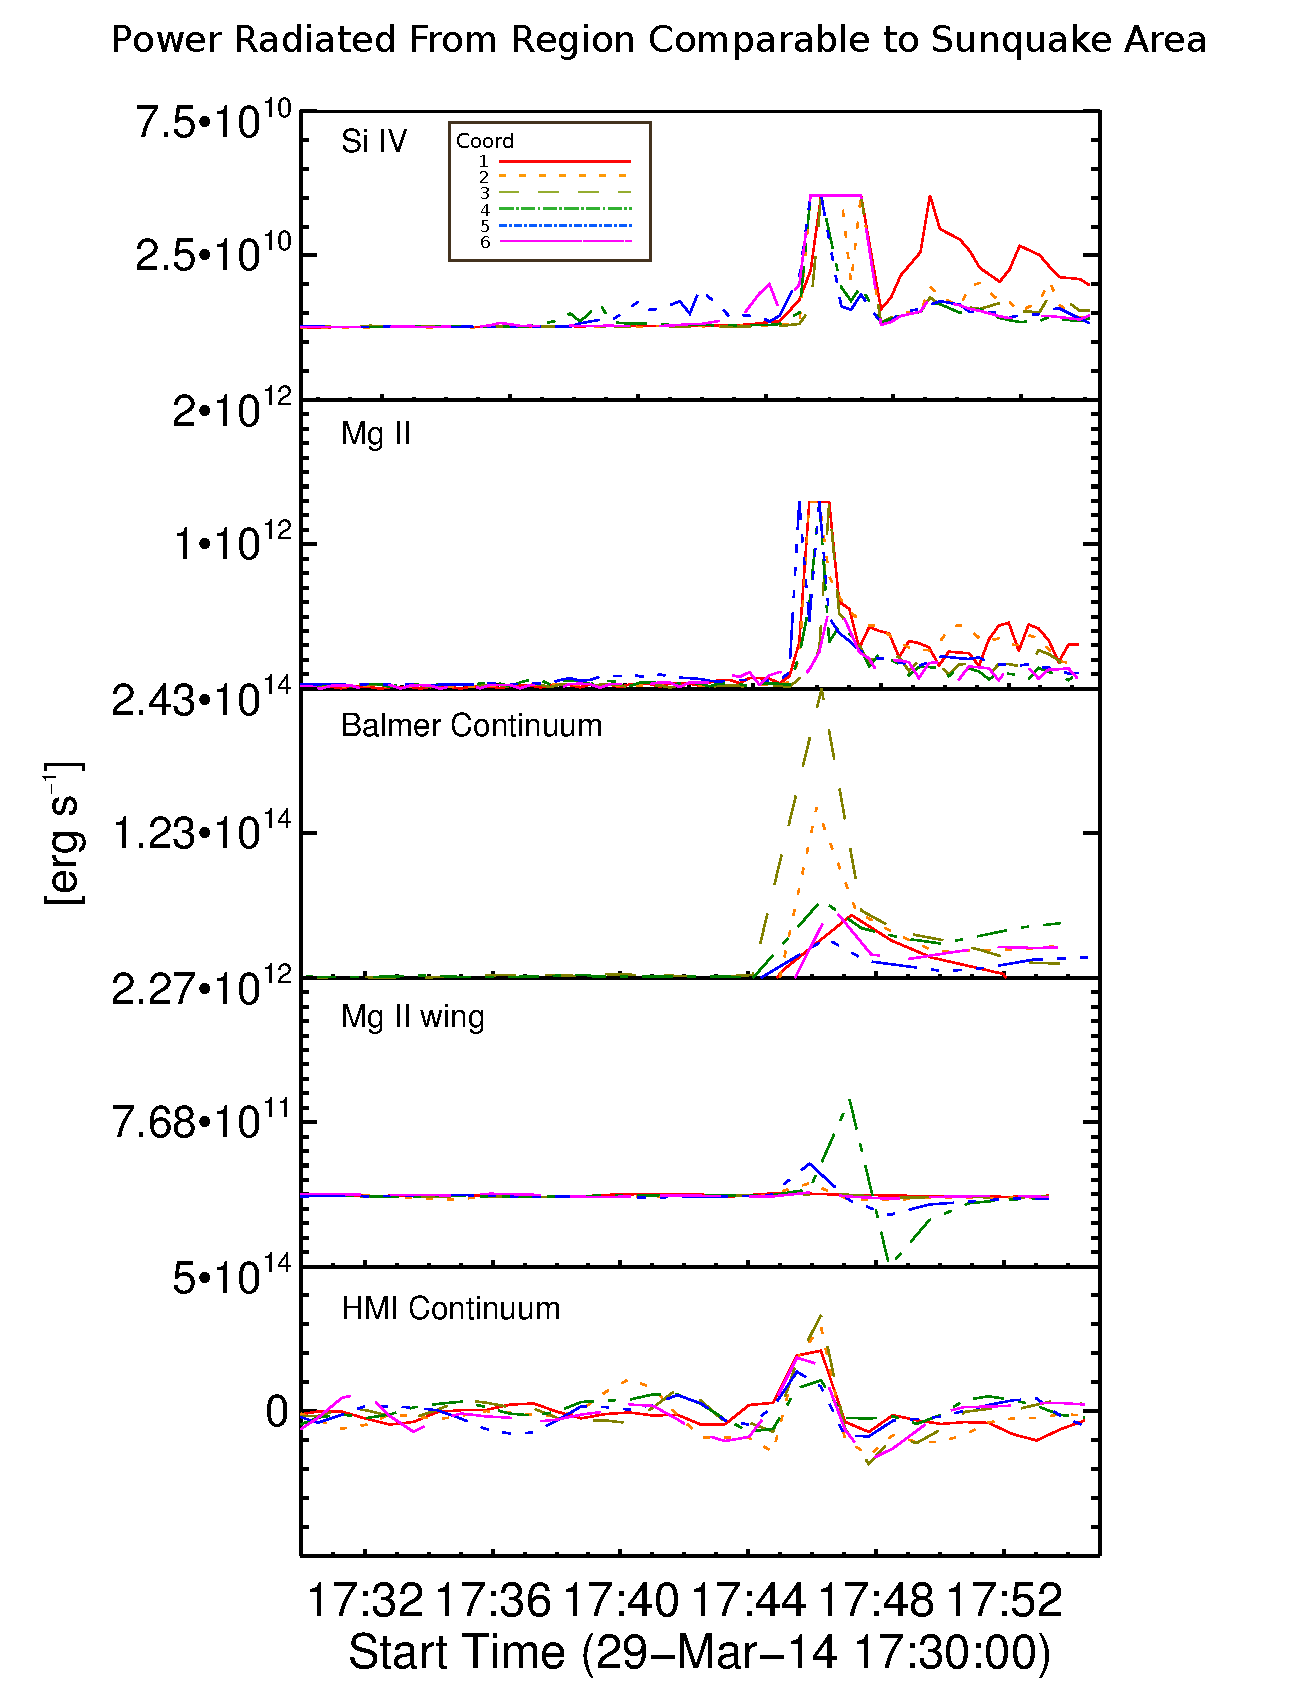
\includegraphics[width=0.6\textwidth]{29-Mar-14-A_sqk-Power-Ladder}
%  \end{center}                                                                                                                                                                                                                                                                                                                                                                                                                                                                                                                                                                                                                                                                                                                                                                                                                                                                                                                                                                                                                                                                                                                                                                                                                                                                                                                                                                                                                                                                                                                                                                                                                                                                                                                                                                                                                                                                                                                                                                                                                                                                                                                                                                                                                                                                                                                                                                                                                                                                                  
%  \caption{Shows radiative power [erg.s$_{-1}$], which is the result of flux data that has been multiplied by the sunquake impact area. The six lines (see legend) represent areas centered on regions 1 to 6, relating to heliocentric coordinates shown in Table \ref{coordtab}. The solid red line is directly over the sunquake location. Each plot represents an independant data set, in order from top to bottom the sets are; IRIS SJ 1400 (Si IV); IRIS SJ 2796 (Mg II); IRIS SG  2825.7 to 2825.8 (Balmer Continuum); IRIS SJ 2832 (Mg II wing); SDO HMI continuum (HMI).}\label{powerladder}
%\end{figure}





